\section{Pre-MVA loose cut-based analysis}

\label{sec:results}

In this section we present the results of the pre-MVA
loose cut-based analysis described in the previous section, and provide 
cut-flows for the different analysis steps.
%
We study how the signal significance
is affected if only the $4b$ component of the
QCD multi-jet background is taken into account.
%
This section presents the results in an environment
without pileup; the following one contains those
obtained including significant PU.

\subsection{Cut-flow and signal significance}

Here we compare the cross-sections for
signal and background events at various
stages of the analysis.
%
We consider all relevant backgrounds (see Sect.~\ref{mcgeneration}),
and discuss how results are modified in the case where only the $4b$
background is considered.
%
In Table~\ref{tab:cutflowdetails}
the different
steps of the cut-flow in the present analysis are summarised,
separated into the boosted, intermediate,
    and resolved topologies.
    %
    The different analysis steps proceed as follows:
   
%%%%%%%%%%%%%%%%%%%%
\begin{table}[t]
  \centering
  \begin{tabular}{|c|c|c|c|}
\hline
&  Boosted  &   Intermediate &  Resolved  \\
\hline
\hline
\multirow{2}{*}{{\bf C1a}} & $N_{\rm jets}^{R10}\ge 2$ & $N_{\rm jets}^{R04}\ge 2$, $N_{\rm jets}^{R10}=1$  &
$N_{\rm jets}^{R04}\ge 4$ \\
 & \multicolumn{3}{c|}{+$p_T$ cuts and rapidity cuts} \\
\hline
\multirow{2}{*}{{\bf C1b}} & +$N_{\rm MDT}\ge 2$ & +$N_{\rm jets}^{R10}=1$ with MDT  &
 +Higgs reconstruction \\
  &  &
 +Higgs reconstruction  & \\
 \hline
{\bf C1c} & \multicolumn{3}{c|}{ +$m_h$ window cut} \\
\hline
{\bf C2} & \multicolumn{3}{c|}{+$b$-tagging}    \\
\hline
  \end{tabular}
  \caption{\small Definition of the cuts imposed successively for the three selections.
    %
      \label{tab:cutflowdetails}
  }
\end{table}
%%%%%%%%%%%%%

\begin{itemize}
     %
    \item {\bf C1a}:  check that we have at least
      two large-$R$ jets (in the boosted case),
      one large-$R$ jet and at least 2 small-$R$ jets (in the intermediate
      case) and at least four small-$R$ jets (in the resolved case).

      In addition,
  require that these jets 
      satisfy the corresponding $p_T$ thresholds;
      $p_T \ge 200$ GeV for large-$R$ jets and
      $p_T \ge 40$ GeV for small-$R$ jets, as well as
      the associated
      rapidity acceptance constraints.
    \item {\bf C1b}: the two leading large-$R$ jets must
      be mass-drop tagged in the boosted category.
      %
      In the intermediate category, the large-$R$ jet
      must also be mass-drop tagged.
      %
    \item {\bf C1c}: after the two Higgs candidates  have been reconstructed,
      their invariant masses are required to lie within a window around $m_H$,
      in particular between 85 and 165 GeV, Eq.~(\ref{higgsmasswindow}).
          \item {\bf C2}: the
            $b$-tagging conditions are
            imposed (see
            Sect.~\ref{sec:btagging}), and the event is categorised exclusively
            into one of the three topologies, according
            to the hierarchy determined in Sect.~\ref{sec:categorisation}.
      \end{itemize}
    Signal and background events satisfying all the analysis cuts up to the
    C2 level
    are then used as input for the MVA training, to be described next
    in Sect.~\ref{sec:mva}.
    
    In Table~\ref{tab:cutflow_noPU_1} we collect
    the values for the signal and background cross-sections
    at the different analysis steps.
    %
    Results are divided into the resolved, intermediate and boosted categories,
    and are inclusive up to the C2 level, where exclusivity is imposed.
    %
In Table~\ref{tab:cutflow_noPU_1} we also  provide the signal over
      background ratio, $S/B$, and the signal
      significance, $S/\sqrt{B}$, corresponding to an integrated
      luminosity of $\mathcal{L}=3$ ab$^{-1}$.
      %
      These are computed either
      taking into account all the background components or
      the $4b$ QCD background only.
        %
      We find that after $b$-tagging, the  $2b2j$ component is
      of the same order of magnitude as the $4b$ component in all categories.
      %
      This implies that the signal significance at the end of the cut-based
      analysis is degraded due to the contribution
      of light and charm jets being mis-identified as $b$-jets.
    
%%%%%%%%%%%%%%%%%%%%%%%%%%%%%%%%%%%%%%%%%%%%%%%%%
\begin{table}[t]
  \centering
  \scriptsize
  \begin{tabular}{|l|cc|cccc|cccc|}
  \hline
\multicolumn{11}{|c|}{Resolved category, $\la n_{\rm PU}\ra=0$}\\
\hline
&  \multicolumn{6}{c|}{Cross-section [fb]} &  &  & &  \\
   &  $hh\to 4b$ &  total bkg  &   $4b$    &  $2b2j$   &   $4j$    &
$t\bar{t}$ &
$S/B_{\rm tot}$ & $S/B_{\rm 4b}$ & $S/\sqrt{B_{\rm tot}}$ & $S\sqrt{B_{\rm 4b}}$ \\
  \hline
  \hline
 C0    & $39$  &   $5.2\cdot 10^9$   & $1.8\cdot 10^6$ & $3.5\cdot 10^8$ & $4.9\cdot 10^9$ & $3.5\cdot 10^5$  & $7.5\cdot 10^{-9}$   &  $2.2\cdot 10^{-5}$  &   0.03   & 1.6        \\
 C1a   & $39$  &   $5.2\cdot 10^9$   & $1.8\cdot 10^6$ & $3.5\cdot 10^8$ & $4.9\cdot 10^9$ & $3.5\cdot 10^5$ &  $7.5\cdot 10^{-9}$   & $2.2\cdot 10^{-5}$   &     0.03   & 1.6       \\
 C1c   & $22$  &   $2.2\cdot 10^8$   & $6.9\cdot 10^4$ & $1.5\cdot 10^7$ & $2.0\cdot 10^8$ & $2.1\cdot 10^5$ &  $1.0\cdot 10^{-7}$  &  $3.2\cdot 10^{-4}$  &  0.08   & 4.6         \\
 C1d   & $22$  &   $2.2\cdot 10^8$   & $6.9\cdot 10^4$ & $1.5\cdot 10^7$ & $2.0\cdot 10^8$ & $2.1\cdot 10^5$ &  $1.0\cdot 10^{-7}$  & $3.2\cdot 10^{-4}$   &  0.08   & 4.6         \\
 C1e   & $63$  &   $4.4\cdot 10^7$   & $1.6\cdot 10^4$ & $3.2\cdot 10^6$ & $4.1\cdot 10^7$ & $8.8\cdot 10^4$ &   $1.4\cdot 10^{-7}$  &  $3.9\cdot 10^{-4}$   &   0.05   & 2.7         \\
 C2    & $1.2$  &   $4.9\cdot 10^3$   & $1.7\cdot 10^3$ & $2.9\cdot 10^3$ & $2.1\cdot 10^2$ & $47$ &            $ 2.5\cdot 10^{-4}$   & $7.1\cdot 10^{-4}$   &   0.97   & 1.6       \\
\hline
\end{tabular}

  $\,$ \\
  \vspace{0.5cm}
  \begin{tabular}{|l|cc|cccc|cccc|}
  \hline
\multicolumn{11}{|c|}{Intermediate category}\\
\hline
&  \multicolumn{6}{c|}{Cross-section [fb]} &  &  & &  \\
   &  $hh\to 4b$ &  total bkg  &   $4b$    &  $2b2j$   &   $4j$    &
$t\bar{t}$ &
$S/B_{\rm tot}$ & $S/B_{\rm 4b}$ & $S/\sqrt{B_{\rm tot}}$ & $S\sqrt{B_{\rm 4b}}$ \\
  \hline
  \hline
 C0      & 39  &   $5.2\cdot 10^9$   & $1.8\cdot 10^6$ & $3.5\cdot 10^8$ & $4.9\cdot 10^9$ & $3.5\cdot 10^5$ &  $7.5\cdot 10^{-9}$   & $2.2\cdot 10^{-5}$   &   $3.0\cdot 10^{-2}$   & 1.6  \\
 C1c     & 6.9  &   $8.4\cdot 10^7$   & $2.1\cdot 10^4$ & $5.3\cdot 10^6$ & $7.9\cdot 10^7$ & $3.3\cdot 10^4$ &  $8.2\cdot 10^{-8}$   & $3.3\cdot 10^{-4}$ &   $4.1\cdot 10^{-2}$   & 2.6 \\
 C1d     & 6.3  &   $5.8\cdot 10^7$   & $1.4\cdot 10^4$ & $3.6\cdot 10^6$ & $5.5\cdot 10^7$ & $3.0\cdot 10^4$ &  $1.1\cdot 10^{-7}$   & $4.6\cdot 10^{-4}$ &   $4.5\cdot 10^{-2}$   & 2.9\\
 C1e     & 1.3  &   $3.5\cdot 10^6$   & $8.7\cdot 10^2$ & $2.1\cdot 10^5$ & $4.3\cdot 10^7$ & $8.8\cdot 10^3$ &  $3.8\cdot 10^{-7}$   & $1.5\cdot 10^{-3}$  &   $3.9\cdot 10^{-2}$   & 2.5\\
 C2      & 0.22  &   $1.8\cdot 10^2$   & $5.6\cdot 10^1$ & $9.6\cdot 10^1$ & $2.2\cdot 10^1$ & 3.1 & $1.3\cdot 10^{-3}$   & $4.0\cdot 10^{-3}$  &   $9.2\cdot 10^{-1}$   & 1.6 \\
\hline
\end{tabular}

  $\,$ \\
  \vspace{0.5cm}
    \begin{tabular}{|l|cc|cccc|cccc|}
  \hline
\multicolumn{11}{|c|}{Boosted category, $\la n_{\rm PU}\ra=0$}\\
\hline
&  \multicolumn{6}{c|}{Cross-section [fb]} &  &  & &  \\
   &  $hh\to 4b$ &  total bkg  &   $4b$    &  $2b2j$   &   $4j$    &
$t\bar{t}$ &
$S/B_{\rm tot}$ & $S/B_{\rm 4b}$ & $S/\sqrt{B_{\rm tot}}$ & $S\sqrt{B_{\rm 4b}}$ \\
  \hline
  \hline
C0      & 39  &   $5.2\cdot 10^9$   & $1.8\cdot 10^6$ & $3.5\cdot 10^8$ & $4.9\cdot 10^9$ & $3.5\cdot 10^5$  &   $7.5\cdot 10^{-9}$   & $2.2\cdot 10^{-5}$  &  $ 3.0\cdot 10^{-2}$   & 1.6 \\
 C1a     & 39  &   $5.2\cdot 10^9$   & $1.8\cdot 10^6$ & $3.5\cdot 10^8$ & $4.9\cdot 10^9$ & $3.5\cdot 10^5$  &   $7.5\cdot 10^{-9}$   & $2.2\cdot 10^{-5}$ &  $ 3.0\cdot 10^{-2}$   & 1.6  \\
 C1c     & 9.4  &   $4.6\cdot 10^7$   & $1.1\cdot 10^4$ & $2.9\cdot 10^6$ & $4.3\cdot 10^7$ & $2.4\cdot 10^4$ &   $2.0\cdot 10^{-7}$   & $8.3\cdot 10^{-4}$ &  $ 7.6\cdot 10^{-2}$   & 4.8 \\
 C1d     & 6.7  &   $3.7\cdot 10^7$   & $7.5\cdot 10^3$ & $2.1\cdot 10^6$ & $3.5\cdot 10^7$ & $2.2\cdot 10^4$ &   $1.8\cdot 10^{-7}$   & $9.0\cdot 10^{-4}$ &  $ 6.0\cdot 10^{-2}$   & 4.2  \\
 C1e     & 2.5  &   $3.9\cdot 10^6$   & $8.0\cdot 10^2$ & $2.3\cdot 10^5$ & $3.7\cdot 10^6$ & $7.1\cdot 10^3$   &   $6.4\cdot 10^{-7}$   & $3.1\cdot 10^{-3}$ &  $ 6.9\cdot 10^{-2}$   & 4.9\\
 C2      & 0.4  &   $2.5\cdot 10^2$   & $5.3\cdot 10^1$ & $1.9\cdot 10^2$ & $1.3\cdot 10^1$ & 1.6  &   $1.4\cdot 10^{-3}$   & $6.7\cdot 10^{-3}$ &   1.2   & 2.7  \\
\hline
\end{tabular}
%%%%%%%%%%%%%%%%%%%%%%%%%%%%%%%%%%%%%%%%%%%%%%%%%%%%%%%%%%%%%%%

    \caption{\small The cross-sections
      for the signal and the background
      processes at different steps of the
      analysis (see Table~\ref{tab:cutflowdetails}), for the resolved (upper),
      intermediate (middle) and boosted
      (lower table) categories, for the analysis
      without PU.
      %
      For each step, the signal over
      background ratio $S/B$, and the signal
      significance $S/\sqrt{B}$ for
       $\mathcal{L}=3$ ab$^{-1}$ are also provided, considering either
      the total background or only the $4b$ component.
      %
 \label{tab:cutflow_noPU_1}}
\end{table}
%%%%%%%%%%%%%%%%%%%%%%%%%%%%%%%%%%%%

%
In the boosted category, at the end of the loose cut-based
analysis, we find that around 500 events
are expected
at the HL-LHC, with a large number,
$\simeq 10^6$, of background events.
%
This leads to a pre-MVA signal significance of
$S/\sqrt{B}=0.5$ and a signal over background
ratio of $S/B=0.06\%$.
%
From Table~\ref{tab:cutflow_noPU_1}
it is also possible to compute the corresponding pre-MVA
expectations for the LHC Run II with
$\mathcal{L}=300$ fb$^{-1}$: one expects in the boosted
category around
50 signal events, with signal significance dropping down to
$S/\sqrt{B}\simeq 0.16$.
%
Such signal
significances could have been enhanced
by applying tighter selection requirements,
but our analysis cuts have been left deliberately loose
so that such optimisation may be performed by the MVA.

The resolved category benefits from higher signal yields,
but this enhancement is compensated for by the
corresponding
increase in the QCD multi-jet background.
%
In both resolved and intermediate categories
the signal significance is
$S/\sqrt{B}\simeq 0.4$,
similar to that of the boosted category.
%
A further
drawback of the resolved case is
that $S/B$
is substantially reduced as compared to the boosted and
intermediate cases.


Combining the results
from the boosted, intermediate and resolved categories,
we obtain an overall pre-MVA 
significance for the observation of the Higgs pair production
in the $b\bar{b}b\bar{b}$ final
state at the HL-LHC 
of  $(S/\sqrt{B})_{\rm tot} \simeq 0.8$.

\subsection{The role of light  and charm jet mis-identification}

One of the main differences in the present study as compared
to previous works is the inclusion of both irreducible
and reducible background components, which allows us to
quantify
the impact of light and charm jet mis-identification. 
%
Two recent studies that have also studied the
feasibility of SM Higgs pair production in the $b\bar{b}b\bar{b}$
final state are from the UCL group~\cite{Wardrope:2014kya} and from
the
Durham group~\cite{deLima:2014dta}.
%
The UCL study is based
on requiring at least four $b$-tagged $R=0.4$ anti-$k_T$ jets
in central acceptance with $p_T \ge 40$ GeV, which are
then used to construct dijets (Higgs candidates) with
$p_T \ge 150$ GeV, $85 \le m_{\rm dijet} \le 140$ GeV
and $\Delta R \le 1.5$ between the two components
of the dijet.
%
In addition to the basic selection cuts, the constraints
from additional kinematic variables are included by means of a 
Boosted Decision Tree (BDT) discriminant.
%
The backgrounds included are the $4b$ and
$2b2c$ QCD multijets, as well as
$t\bar{t}$, $Zh$, $t\bar{t}h$ and $hb\bar{b}$.
%
For the HL-LHC, a signal significance of $S/\sqrt{B}\simeq 2.1$ 
is obtained.

The Durham group study~\cite{deLima:2014dta} requires events
to have two $R=1.2$ C/A jets with $p_T\ge 200$ GeV, and in
addition
two $b$-tagged subjets inside each large-$R$ jet with
$p_T \ge$ 40 GeV each.
%
To improve the separation between
signal and background, both the BDRS
method and the Shower Deconstruction (SD)~\cite{Soper:2011cr,Soper:2012pb}
technique are used.
%
The backgrounds considered are QCD $4b$ as well as $Zb\bar{b}$, $hZ$ and
$hW$.
%
At the HL-LHC, their best result is obtained by requiring two
SD-tagged large-$R$ jets, which leads to $S/\sqrt{B}\simeq 2.1$.
%
Using the BDRS tagger
results in slightly poorer performance.
 %
 
 From our results in Table~\ref{tab:cutflow_noPU_1}, we observe
 that the signal significance for the boosted, intermediate,
 and resolved categories is increased to 1.1, 0.6 and 0.6, respectively,
 when only the QCD $4b$ background is included.
 %
 Combining
 the signal significance in the three categories,
 we
 obtain $(S/\sqrt{B_{\rm 4b}})_{\rm tot}\simeq 1.4$, twice
 as large as the result found when
 all background components are included.
 %
 Note the importance of
 the combination of the three exclusive event topologies,
 as opposed the exploitation of a single specific category.
 %
 Taking into account the loose selection cuts, we
 see that
 our pre-MVA results including only the $4b$ background are consistent
 with those reported in previous studies.

 From Table~\ref{tab:cutflow_noPU_1} we
 can compare the interplay
 between the reducible and irreducible components of the
 QCD backgrounds.
 %
 In all cases, the $4b$ and $2b2j$ components have comparable
 magnitudes within the uncertainties from missing higher-order
 corrections.
 %
 On the other hand, the $4j$ component
is always substantially smaller.
 %
  So while the $4j$ component can be safely
 neglected, the inclusion of the
 $2b2j$ component is essential to assess the feasibility
 of measuring Higgs pairs in this final state robustly,
 especially
 in the boosted category.
 %
 This has the important
 consequence that a promising avenue to improve the prospects
 of this measurement would be to reduce, as much as possible,
 the light and charm jet mis-identification rate.

 In Fig.~\ref{fig:histoBack} we show a
 comparison
    of the shapes of the $4b$ and $2b2j$
    components of the QCD background for the transverse momentum
    $p_T^h$ of the leading
Higgs candidate and for invariant
mass $m_{hh}$ of the
    reconstructed di-Higgs system in the resolved
    and boosted  categories.
     %
    The two components possess a rather similar shape
    for the two distributions, albeit with some 
    differences.
  %
    In the boosted
    category, the $4b$ component exhibits a less steep fall-off of
    the $p_T^h$ distribution at large $p_T$,
    while in the resolved case
    the $2b2j$ component has a slightly harder
    distribution of the  invariant
    mass $m_{hh}$.
%
    We also observe that the $2b2j$ distributions
    are affected by somewhat larger
    Monte Carlo fluctuations as compared to $4b$, despite the large size
of the initial sample.
%

%%%%%%%%%%%%%%%%%%%%%%%%%%%%
\begin{figure}[t]
\begin{center}
 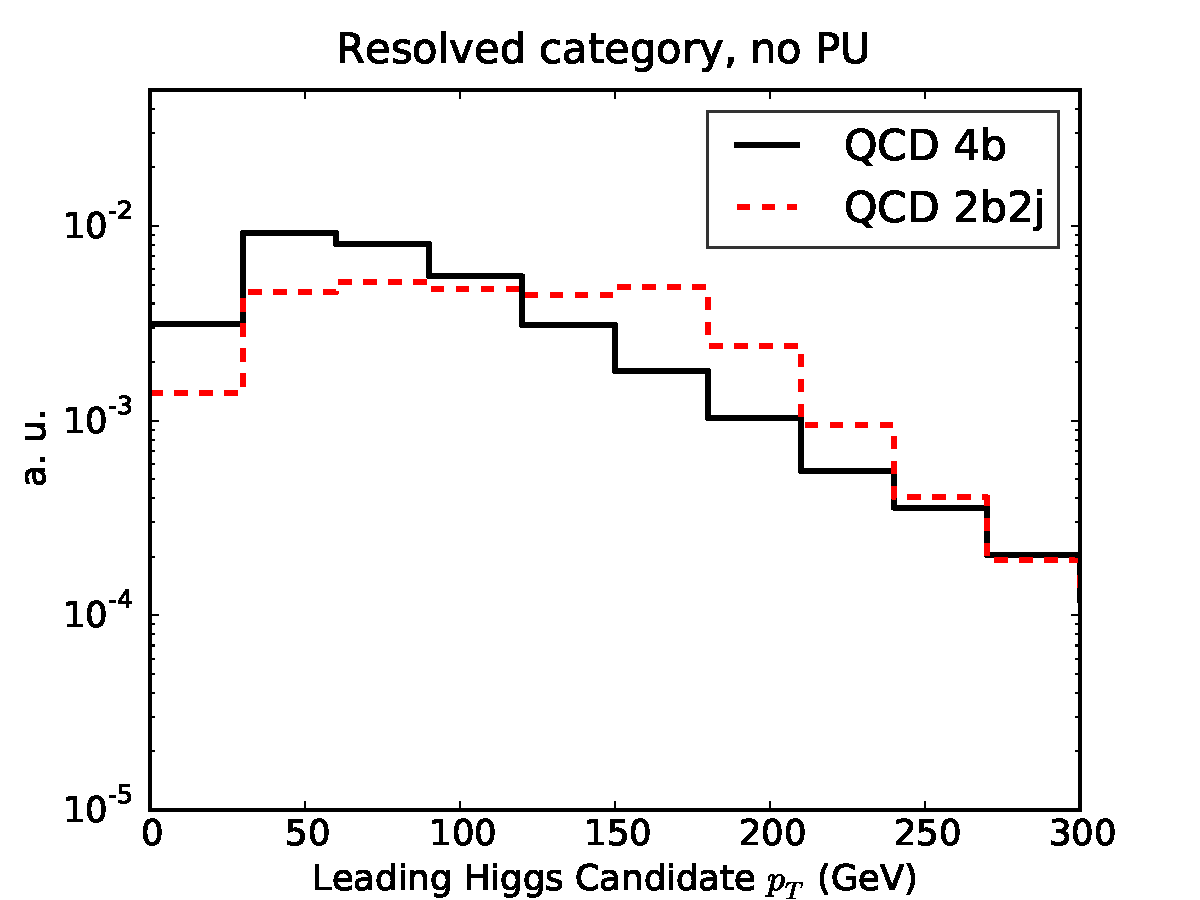
\includegraphics[width=0.49\textwidth]{plots/pt_h0_C2_res_back_noPU.pdf}
 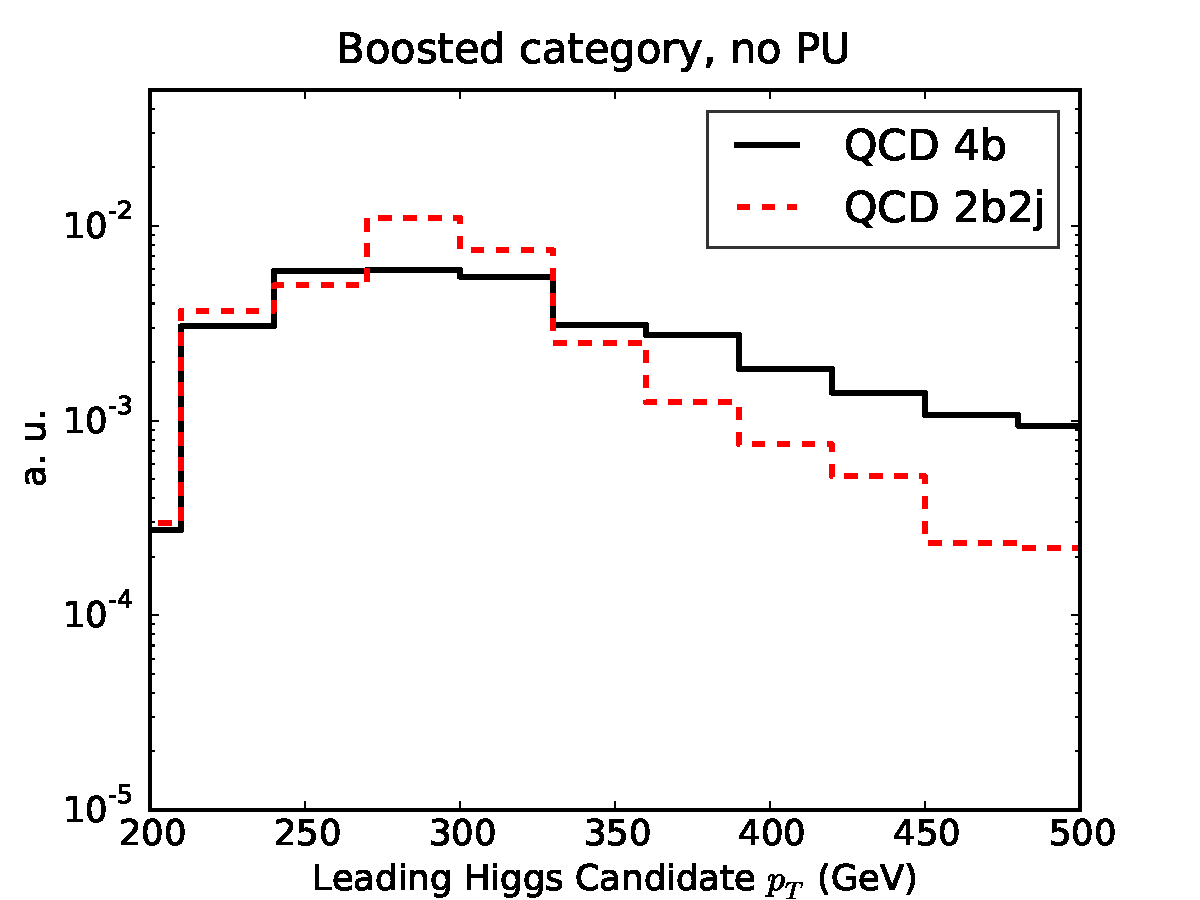
\includegraphics[width=0.49\textwidth]{plots/pt_h0_C2_bst_back_noPU.pdf}
  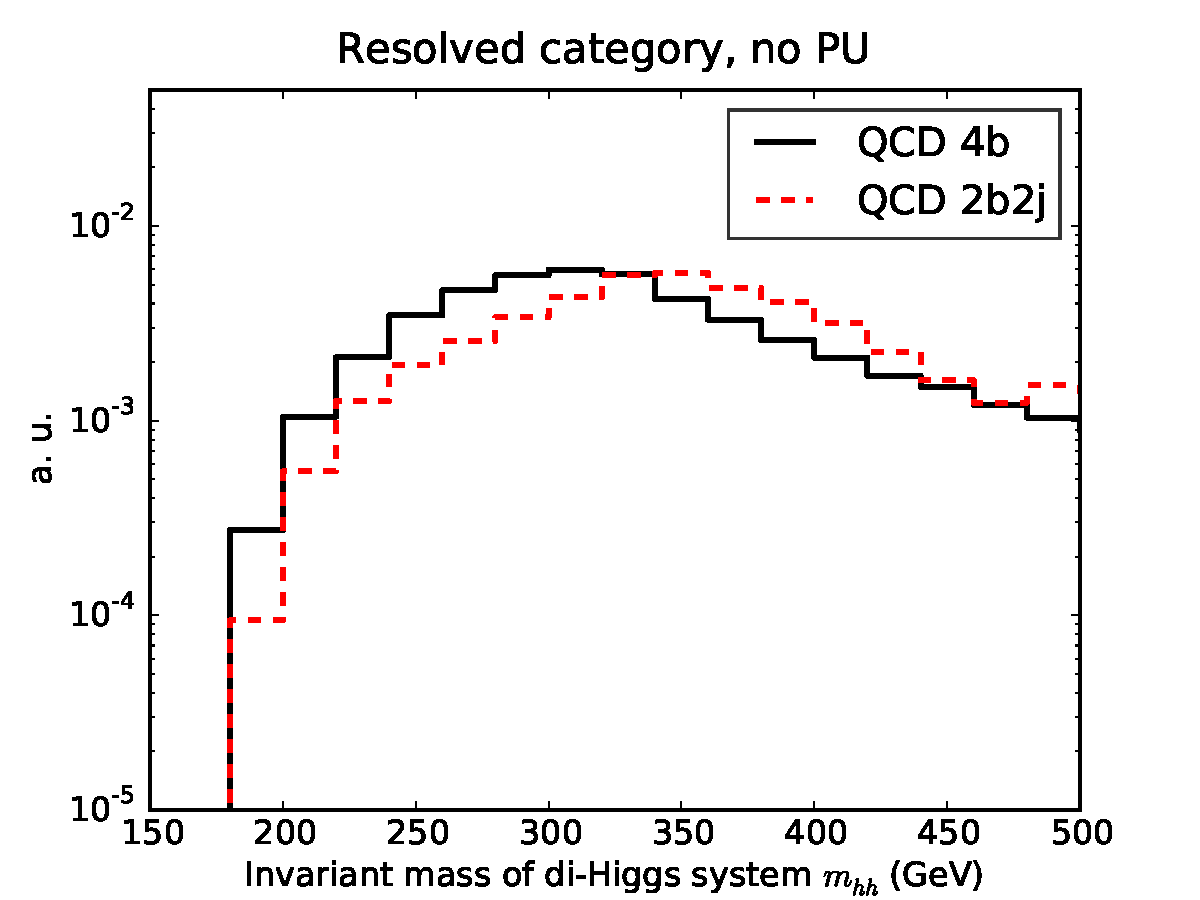
\includegraphics[width=0.49\textwidth]{plots/m_hh_C2_res_back_noPU.pdf}
  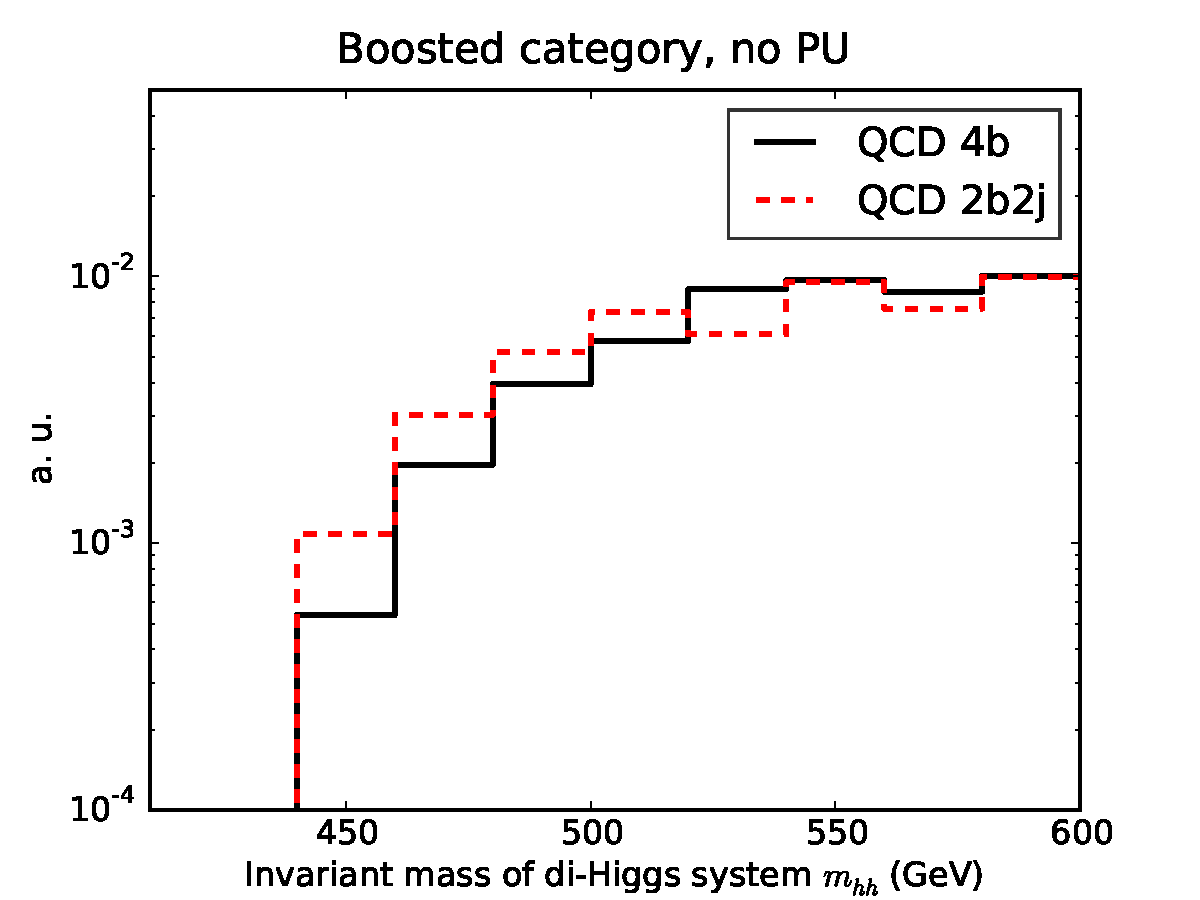
\includegraphics[width=0.49\textwidth]{plots/m_hh_C2_bst_back_noPU.pdf}
  \caption{\small
    Upper plots: comparison
    of the shapes of the $4b$ and $2b2j$
components of the QCD background for the $p_T^h$ of the leading
Higgs candidate in the resolved
(left plot) and boosted (right plot) categories.
    %
Lower plots:  same comparison for the invariant
mass $m_{hh}$ of the
    reconstructed di-Higgs system.
}
\label{fig:histoBack}
\end{center}
\end{figure}
%%%%%%%%%%%%%%%%%%%%%%%

In the resolved category, 
the cross-section  before
$b$-tagging is two orders
of magnitude larger in the $2b2j$
sample as compared to the $4b$ sample.
%
After $b$-tagging, a naive assessment would
suggest a suppression of the $2b2j$ cross-section by a factor $(f_l/f_b)^2 \simeq
1.5\cdot 10^{-4}$, as compared to the $4b$ component,
since a total of four $b$-tags are required to classify the
event as a Higgs candidate.
%
In this case the ratio of $2b2j$ over $4b$ would be
around $\simeq 3\%$, and therefore negligible.
  %
While  we have checked that this expectation is borne
out at the parton level,
we find that  when parton shower effects
are accounted for the situation is different, due both to radiation of $b\bar{b}$ pairs
and from selection effects.
%
Due to these,
the
number of  $b$ quarks in the  final state is
increased substantially in the $2b2j$ component as compared
to the parton level, while at the same
time the number of events in the $4b$ sample
with 4 $b$-jets passing selection cuts is reduced.

We can make these statements more quantitative in the following way.
%
To first approximation, neglecting the contribution from
charm mis-identification,
the
overall efficiency of the $b$-tagging requirements in the resolved category will be
given by the following expression:
\be
\label{btaggingeff}
{\rm EFF}_{\rm b-tag}\simeq \sum_{j=0}^{4}n^{\rm (b-jet)}_j\cdot f_b^{j}\cdot f_l^{4-j} \, ,
\ee
with $n^{\rm (b-jet)}_j$ being the fraction of events satisfying all the selection
requirements,
where $j$ jets out of the leading four jets of the event
contain $b$ quarks (with $p_T^b\ge 15$
GeV).
%
Similar expressions can be derived for
the boosted and intermediate categories.
%

The naive expectation is that all events in the $4b$ sample have $n^{\rm (b-jet)}_4\simeq 1$
and $n^{\rm (b-jet)}_j\simeq 0$ for $j\ne 4$, while the events in the $2b2j$ sample
should have $n^{\rm (b-jet)}_2\simeq 1$ and zero otherwise.
%
This leads to a ratio of overall $b$-tagging selection efficiencies
\be
\label{eq:naive}
\frac{ {\rm EFF}_{\rm b-tag} \lc 2b2j \rc}{{\rm EFF}_{\rm b-tag} \lc 4b\rc}
  \simeq
 \lp \frac{f_l}{f_b}\rp^2 \simeq 1.5\cdot 10^{-4} \, .
\ee
However, after the parton shower, the above estimate is no longer accurate.
%
First of all, we will have a non-negligible fraction $n^{\rm (b-jet)}_j$
with $j=3,4$ also in the $2b2j$ sample, due to $b$-quark pair radiation
during the shower.
%
Secondly, not all events in the $4b$ sample will lead to four small-$R$ $b$-jets,
due to a combination of selection cuts and
parton shower effects.
%

%%%%%%%%%%%%%%%%%%%%%%%%%%%%%%%%%%%%%%%%%%%%%%%%
\begin{table}[t]
  \centering
  \small
  \begin{tabular}{|c|c|c|c|c|c|c|c|}
    \hline
  \multicolumn{2}{|c|}{}   &  $n^{\rm (b-jet)}_0$  &  $n^{\rm (b-jet)}_1$  &  $n^{\rm (b-jet)}_2$  & $n^{\rm (b-jet)}_3$ &
    $n^{\rm (b-jet)}_4$ & ${\rm EFF}_{\rm b-tag}$ \\
    \hline
    \hline
    Signal  &  $hh\to 4b$  &   0.1\%    & 3\%     &  25\%     & 53\%     & 20\%      & 8.5\%  \\
    \hline
    \multirow{3}{*}{Background}  &  QCD $4b$  & 1\%      &  8\%    &   27\%   &  44\%     & 20\%       &  8.4\% \\
     &  QCD $2b2j$  &   9\%    & 42\%     &  49\%    & 1\%     &  0.1\%     & 0.04\%  \\
    &  QCD $4j$  &   96\%    &  3.5\%     & 0.5\%     &  0.01\%    & $3\cdot 10^{-4}$\%      &
    $2\cdot 10^{-4}$\%\\
    \hline
  \end{tabular}
  \caption{\small
    The relative fractions  $n^{\rm (b-jet)}_j$ of events for the resolved selection
    for which out of the four leading small-$R$ jets of the
    event, $j$ jets
    contain at least one $b$-quark with $p_T^b\ge 15$ GeV.
    %
    This information is provided
    for the di-Higgs signal events and for the three QCD background samples.
    %
    The last column indicates the overall 
    selection efficiency as defined in
    Eq.~(\ref{btaggingeff})
    \label{tab:btaggingcheck}
  }
  \end{table}
%%%%%%%%%%%%%%%%%%%%%%%%%%%%%%%%%%%%%%%%%%%%%%%

In Table~\ref{tab:btaggingcheck} we collect
the values of $n^{\rm (b-jet)}_j$ for the signal and the three QCD background samples.
%
We find that rather than the estimate Eq.~(\ref{eq:naive}),
the correct ratio of $b$-tagging selection efficiencies is instead
\be
\frac{{\rm EFF}_{\rm b-tag} \lc 2b2j\rc}{{\rm EFF}_{\rm b-tag} \lc 4b\rc}=
  \frac{0.04\%}{8.4\%} \simeq 5\cdot 10^{-3} \, .
  \ee
  This suppression factor is of the same order as
  the ratio of $4b$ to $2b2j$ cross-sections
  in the resolved category before $b$-tagging.
    %
    This explains why the $2b2j$ contribution cannot be neglected as compared
    to the irreducible $4b$ component of the QCD background.
    %
    A similar calculation from the numbers in Table~\ref{tab:btaggingcheck}
    shows
    that, on the other hand, the $4j$ component of the background
    can be neglected.

    
